\documentclass[
  bibliography=totoc,     % Literatur im Inhaltsverzeichnis
  captions=tableheading,  % Tabellenüberschriften
  titlepage=firstiscover, % Titelseite ist Deckblatt
]{scrartcl}

% Paket float verbessern
\usepackage{scrhack}

% Warnung, falls nochmal kompiliert werden muss
\usepackage[aux]{rerunfilecheck}

% unverzichtbare Mathe-Befehle
\usepackage{amsmath}
% viele Mathe-Symbole
\usepackage{amssymb}
% Erweiterungen für amsmath
\usepackage{mathtools}

% Fonteinstellungen
\usepackage{fontspec}
% Latin Modern Fonts werden automatisch geladen
% Alternativ zum Beispiel:
%\setromanfont{Libertinus Serif}
%\setsansfont{Libertinus Sans}
%\setmonofont{Libertinus Mono}

% Wenn man andere Schriftarten gesetzt hat,
% sollte man das Seiten-Layout neu berechnen lassen
\recalctypearea{}

% deutsche Spracheinstellungen
%\usepackage[ngerman]{babel}


\usepackage[
  math-style=ISO,    % ┐
  bold-style=ISO,    % │
  sans-style=italic, % │ ISO-Standard folgen
  nabla=upright,     % │
  partial=upright,   % ┘
  warnings-off={           % ┐
    mathtools-colon,       % │ unnötige Warnungen ausschalten
    mathtools-overbracket, % │
  },                       % ┘
]{unicode-math}

% traditionelle Fonts für Mathematik
\setmathfont{Latin Modern Math}
% Alternativ zum Beispiel:
%\setmathfont{Libertinus Math}

\setmathfont{XITS Math}[range={scr, bfscr}]
\setmathfont{XITS Math}[range={cal, bfcal}, StylisticSet=1]

% Zahlen und Einheiten
\usepackage[
  locale=DE,                   % deutsche Einstellungen
  separate-uncertainty=true,   % immer Unsicherheit mit \pm
  per-mode=symbol-or-fraction, % / in inline math, fraction in display math
]{siunitx}

% chemische Formeln
\usepackage[
  version=4,
  math-greek=default, % ┐ mit unicode-math zusammenarbeiten
  text-greek=default, % ┘
]{mhchem}

% richtige Anführungszeichen
\usepackage[autostyle]{csquotes}

% schöne Brüche im Text
\usepackage{xfrac}

% Standardplatzierung für Floats einstellen
\usepackage{float}
\floatplacement{figure}{htbp}
\floatplacement{table}{htbp}

% Floats innerhalb einer Section halten
\usepackage[
  section, % Floats innerhalb der Section halten
  below,   % unterhalb der Section aber auf der selben Seite ist ok
]{placeins}

% Seite drehen für breite Tabellen: landscape Umgebung
\usepackage{pdflscape}

% Captions schöner machen.
\usepackage[
  labelfont=bf,        % Tabelle x: Abbildung y: ist jetzt fett
  font=small,          % Schrift etwas kleiner als Dokument
  width=0.9\textwidth, % maximale Breite einer Caption schmaler
]{caption}
% subfigure, subtable, subref
\usepackage{subcaption}

% Grafiken können eingebunden werden
\usepackage{graphicx}

% schöne Tabellen
\usepackage{booktabs}

% Verbesserungen am Schriftbild
\usepackage{microtype}

% Keine Einrueckungen nach Absatz
\setlength{\parindent}{0pt}

% Lange Tabellen schoen
\usepackage{longtable}

% Literaturverzeichnis
\usepackage[
  backend=biber,
]{biblatex}
% Quellendatenbank
\addbibresource{lit.bib}
\addbibresource{programme.bib}

% Hyperlinks im Dokument
\usepackage[
  german,
  unicode,        % Unicode in PDF-Attributen erlauben
  pdfusetitle,    % Titel, Autoren und Datum als PDF-Attribute
  pdfcreator={},  % ┐ PDF-Attribute säubern
  pdfproducer={}, % ┘
]{hyperref}
% erweiterte Bookmarks im PDF
\usepackage{bookmark}

% Trennung von Wörtern mit Strichen
\usepackage[shortcuts]{extdash}

\author{%
  Theodor Zies\\%
  \href{theodor.zies@tu-dortmund.de}{theodor.zies@tu-dortmund.de}%
  \and%
  Can Toraman\\%
  \href{can.toraman@tu-dortmund.de}{can.toraman@tu-dortmund.de}%
}
\publishers{TU Dortmund – Physics department}

\subject{Advanced labaratory course}
\title{Selection of \texorpdfstring{$B_s \to \psi(2S)K_s$}{B_s -> Psi(2S)K_S} decays using a multivariate analysis}
\date{%
  Colloqium: 07.07.2024
  \hspace{3em}
  Hand-in: xx.xx.xxx
}
\newcommand{\signal}{$B_s \to \psi(2S)K_s$}

\usepackage{tikz}
\usepackage{tikz-feynman}
\usepackage{amsmath}


\begin{document}

\maketitle
\thispagestyle{empty}
\tableofcontents
\newpage

\section{Objective}
\label{sec:Obj}
The objective of this experiment is to understand the workings of a silicone strip detector and its properties. Additionally, the use of readout electronics and resulting data is supposed to further introduce the participant into their usage in different detector systems.
\section{Theory}
\label{sec:Theo}

In order to understand a silicone strip detector it is important to look at the theory of semiconductors.
\subsection{Semiconductors}
Semiconductors are defined by the energy gap of the valence and conduction band. If the bands overlap in a material it is referred to as \textit{conductor} since the electrons can move freely in the material. If the energy gap is to great the electrons can't travel into the conduction band, therefore these materials are called \textit{insulators}. If though the energy gap is in the range below \qty{3}{\eV} the material is a \textit{semiconductor}. The semiconductor employed in this experiment is silicone with a band gap of \qty{1.107}{\eV} \cite{V15}. Silicone has four valence electrons and arranges itself in a diamond lattice structure. One of the properties of a semiconductor is, if the valence electrons are exited e.g. thermal effects or other external particles, it creates a hole in the valence band, which can be treated as a quasi particle with a negative charge. The electron and hole can form a bound state resembling an atom, if the material is placed into a electric field (e.g. by placing a cathode/anode to the materiel) the formation of such a state is prevented. The electrons and holes can now travel to the cathode/anode. This behavior can be modified by a process called \textit{doping}, in which some of the silicone particles in the crystalline structure are replaced by elements that carry a higher/lower amount of valence electrons. %auch noch bild einfuegen

\subsubsection{n-type semiconductor}

If the element used for doping has a valence charge higher than four (e.g. Arsenic: five valence electrons), one electron is not used for the binding in the crystalline structure so it can move almost freely in the material. 

\subsubsection{p-type semiconductor}
Analog to the n-type semiconductor the introduced material has fewer electrons in its valence band (Boron: three valence electrons). The boron would then leave one of the bonds to the it surrounding silicone atoms partially empty creating a hole, which then can move freely like the electron. 


\begin{figure}[H]
	\centering
	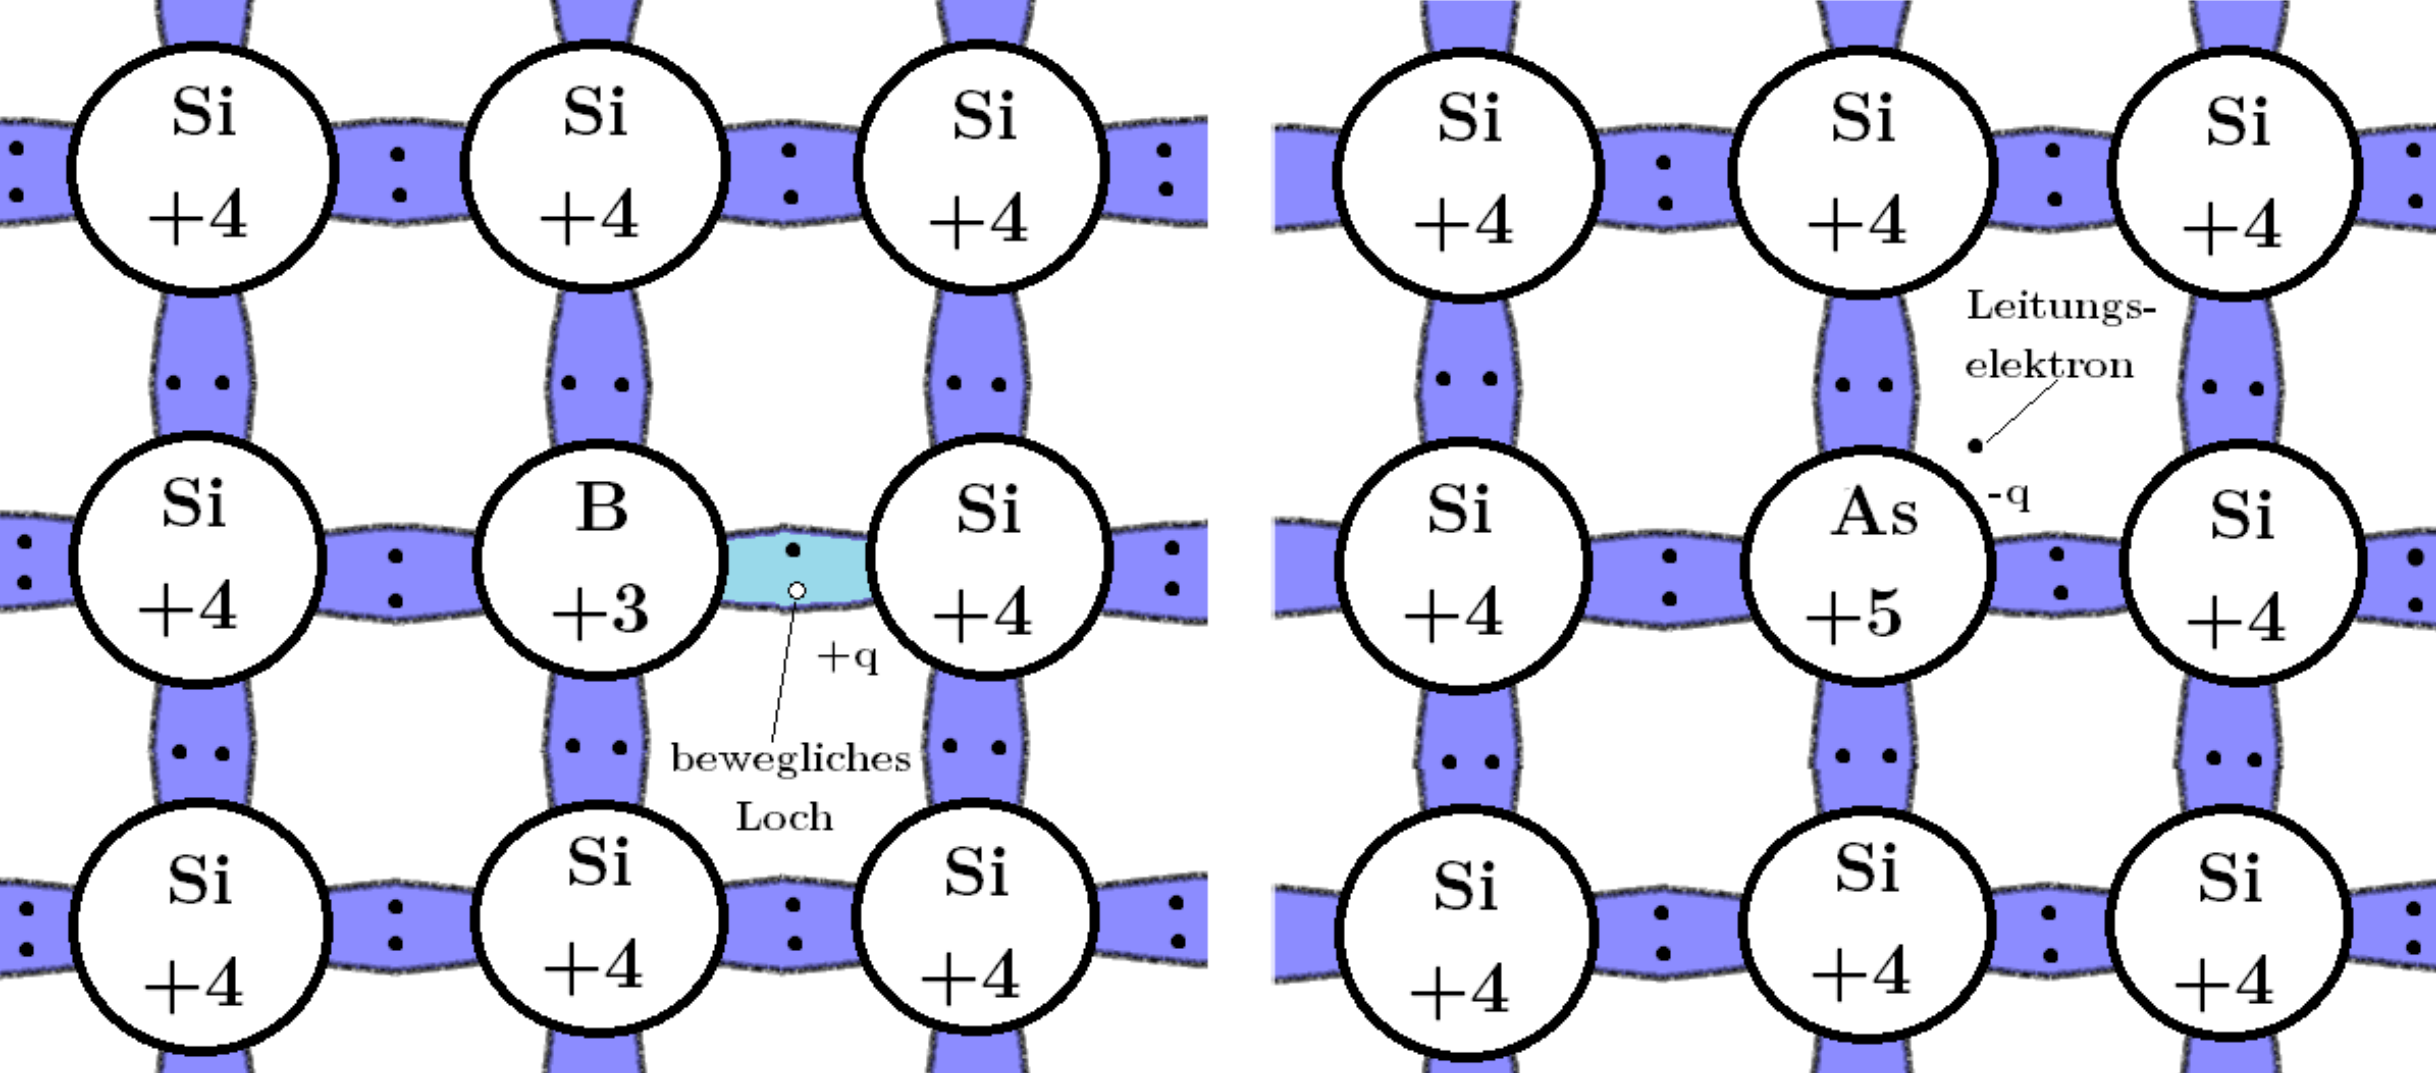
\includegraphics[width=0.7\linewidth]{Assets/doting.png}
	\caption{Graphical representation of boron and arsenic doping in silicone\cite{V15}.}
	\label{fig:doting}
\end{figure}


\subsubsection{pn transition}
If one connects a p and n doped material together so called a diode is created. % This pn transition is the bas
Inside the diode the additional electrons from the n-side now want to recombine with the holes from the p-side. This results in a positive charge on the n-side and a negative on the p-side. The resulting difference of a few \unit{\milli\volt} is called diffusion voltage $U_\mathrm{D}$ \cite{V15}. \\

For the detection of ionizing particles a voltage is applied to either side of the diode, the electrons coming from the applied potential are then recombining with the holes on the p-side and the electron in the n-side flow into the anode, resulting in a zone in which no free charge carriers remain. This zone is called the \textit{depletion zone} and its dimension can be determined to be
\begin{equation}
	d(U) = \sqrt{\frac{2\epsilon(U_\mathrm{D}+ U)}{eN_\mathrm{eff}}},
	\label{depl}
\end{equation}
where U is the voltage applied to the diode, $\epsilon$ the dielectric constant of silicone, $e$ the elementary charge and $N_\mathrm{eff}$ the effective charge carrier density. $N_\mathrm{eff}$ is determined by 
\begin{equation*}
	N_\mathrm{eff} = \frac{N_\mathrm{D}N_\mathrm{A}}{N_\mathrm{D}+N_\mathrm{A}},
\end{equation*}
where $N_\mathrm{D}$,$N_\mathrm{A}$ are the respective densities of the n and p doped materials. When the depletion zone is as large as the diode itself, one speaks of a full depletion at the depletion voltage $U_\mathrm{dep}$. Using the fact that $U\ll U_\mathrm{D}$ it can be determined that $U_\mathrm{dep}$ is given by
\begin{equation*}
	U_\mathrm{dep} \approx \frac{e}{2\epsilon} N_\mathrm{eff} D^2
\end{equation*}
with the thickness of the diode $D$. If the applied voltage is below the depletion voltage then the distance $d_\mathrm{c}(U)$ can be approximated with

\begin{equation*}
	d_\mathrm{c}(U)= D\sqrt{\frac{U}{U_\mathrm{depl}}}.
\end{equation*}
Ideally, the diode is fully depleted so the signal generated by an ionizing particle can be detected. This is not the case since thermal effects an electron can enter the current band and create the so called \textit{leakage current}. This effect increases with higher voltages. The relation between the current and voltage can be seen in \autoref{fig:leackage}.

\begin{figure}[H]
	\centering
	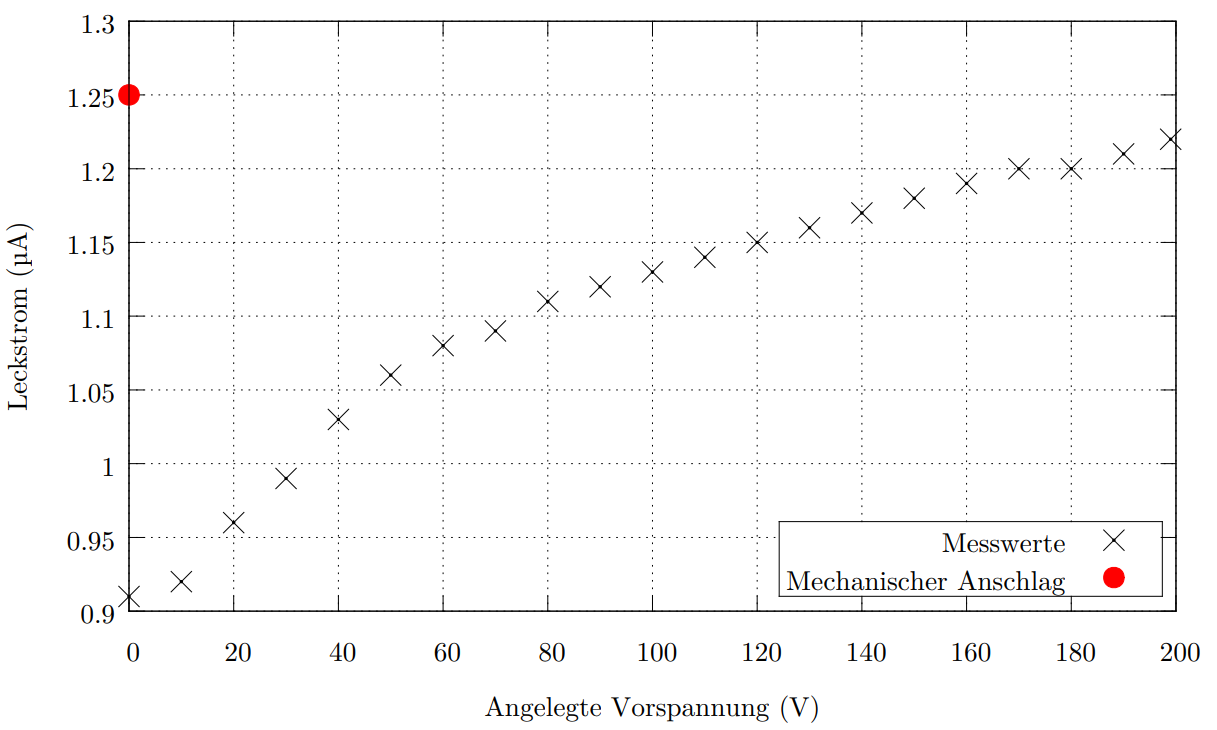
\includegraphics[width=0.7\linewidth]{Assets/leackage}
	\caption{Current measured across the sensor in relation to the applied voltage \cite{V15}.}
	\label{fig:leackage}
\end{figure}


Using this plot the depletion voltage can be determined as the voltage at which the leakage current only increases linearly.

\subsection{Ionizing radiation}
The silicone strip detector can be used to detect ionizing particles. During the experiment a source producing beta particles is employed.
\subsubsection{Beta decay}
The used source is the strontium isotope \ce{^{90}Sr}, which decays via a $\beta^-$ decay into yttrium (maximal energy \qty{0.545}{\mega\eV}), that intern decays into zirconium (maximal energy \qty{2.28}{\mega\eV}) \cite{V15}.
\begin{equation*}
	\ce{^{90}Sr} \rightarrow \ce{^{90}Y} \rightarrow \ce{^{90}Zr}
\end{equation*}

During a $\beta^-$ decay a neutron in the atomic nucleus decays into a proton, electron and an anti-electron-neutrino. Since this process is a three body decay the electron is not produced at a fixed energy. The energy of the emitted electron follows the distribution shown in \autoref{fig:edist}


\begin{figure}[H]
	\centering
	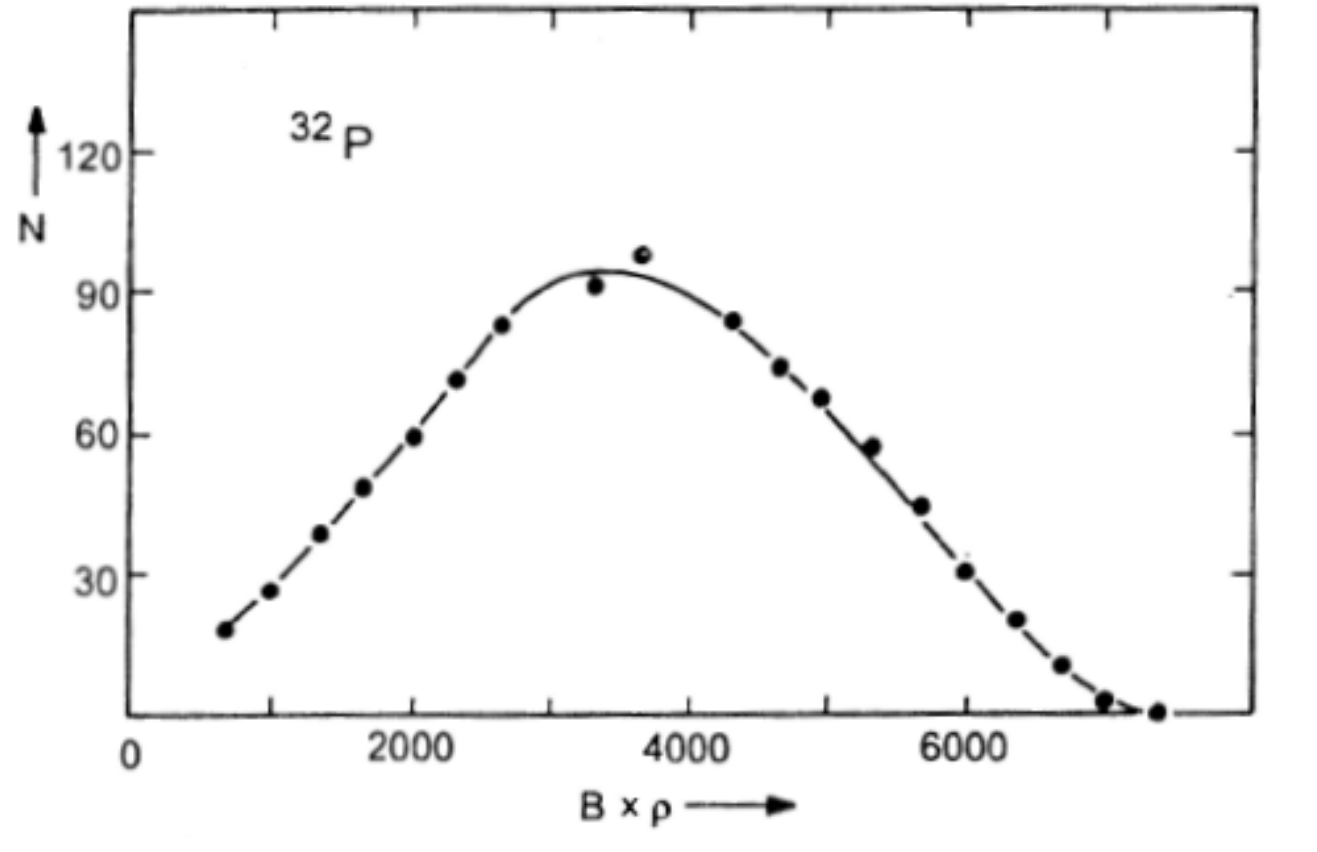
\includegraphics[width=0.7\linewidth]{Assets/edist.png}
	\caption{Energy distribution of a electron originating from ab $\beta^-$ decay \cite{V15}.}
	\label{fig:edist}
\end{figure}

The activity is defined as the rate of change of the number of nuclei $A = - \dot{N}$. From this it can be deduced that the activity can be written as

\begin{equation*}
	A = \lambda N_0 \exp(-\lambda t) = A_0 \exp(-\lambda t),
\end{equation*}
where $A_0$ and $N_0$ are the activity and number of nuclei at $t=0$, and $\lambda$ is the decay constant of the decaying material/particle.

\subsubsection{Interaction in matter}
Due to the energy of the electrons almost only their collisions with the nuclei in the matter it is traversing are contributing to the energy loss. The ionizing particles inside the detector are detected by these collision, as they excite the electrons in the crystalline structure of the detector material. These exited electron then create a measurable signature in the detector. The energy deposited by the electrons can be determined using the Bethe-Bloch equation with additional correction terms:
\begin{equation*}
	-\frac{\mathrm{dE}}{\mathrm{d}x} = 2\pi N_{\mathrm{a}} m_e c \rho \frac{Z}{A} \frac{1}{\beta^2} \left[ln\left(\frac{\tau(\tau+2)}{2(I/m_ec^2)^2}\right)+F(\tau) - \delta - 2\frac{C}{Z}\right],
\end{equation*}
with 
\begin{equation*}
	F(\tau) = 1 - \beta^2 + \frac{\frac{\tau}{8}+(2r_e +1 )\ln(2)}{(\tau+1)^2}, \hspace{0.5cm} \mathrm{where}\hspace{0.2cm} \tau = \gamma-1.
\end{equation*}
The meaning of the symbols and their values can be seen in \cite{V15}.
From this formula it can be determined that the electron originating from the \ce{^{90}Sr} source is depositing \qty{3.88}{\mega\eV} per \unit{\centi\meter} \cite{V15}.\\

Usually for particles traversing a silicone detector the deposited energy can be approximated by a Gaussian distribution. As for a thinner detector (e.g. like the \qty{300}{\micro\meter} of the detector used in this experiment) the thickness is not sufficient enough for the energy loss to be described as Gaussian. The actual distribution is much better described by a Landau distribution. Another effect at play stems from the already described energy distribution of the emitted electron. This results in a convoluted Landau distribution shown in \autoref{fig:landau}.


\begin{figure}[H]
	\centering
	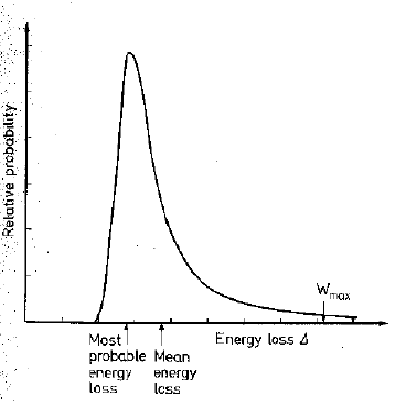
\includegraphics[width=0.45\linewidth]{Assets/landau}
	\caption{Convoluted Landau distribution \cite{V15}.}
	\label{fig:landau}
\end{figure}


\subsection{Noise and pedestals}
As most electronics and detectors can't operate a hundred percent clean, there will always remain noise, signals that interfere with the intended measurement. So the recorded counts from the Analog-Digital-Converter (ADC) can be described by

\begin{equation*}
	\mathrm{ADC}(i,k) = \mathrm{P}(i) + \mathrm{D}(k) + \mathrm{Signal}(i,k),
\end{equation*}
ADC is the probability for a signal $k$ at the $i$-th strip on the detector. $\mathrm{P}(i)$ is the so called \textit{pedestal}. It is determined as the mean value of the $\mathrm{ADC}(i,k)$ without $\mathrm{Signal}(i,k)$. So $\mathrm{P}(i)$ calculated for $N$ measurements as 
\begin{equation}
	\mathrm{P}(i) = \frac{1}{N} \sum_{k=1}^{N}\mathrm{ADC}(i,k).
	\label{eq:pedestal}
\end{equation}
The $\mathrm{D}(k)$ contribution is the \textit{common mode shift} and is calculated using 
\begin{equation}
	\mathrm{D}(k) = \frac{1}{128}\sum_{i=1}^{128}(\mathrm{ADC}(i,k) - \mathrm{P}(i))
	\label{eq:common_mode}
\end{equation}
From these distributions using the root mean square the noise is determined:
\begin{equation}
	\mathrm{Noise}(i)=\sqrt{\frac{1}{N-1}\sum_{k=1}^{N}(\mathrm{ADC}(i,k) - \mathrm{P}(i) - \mathrm{D}(k))^2}
	\label{eq:noise}
\end{equation}
\section{Experimental setup}
The experimental setup consists of a control unit, the detector unit and a computer with a application for the visualization and data taking. The control unit is connected to the detector unit using a ribbon cable and to the computer via a USB connection. Located on the control and detector unit is a glass fiber connection that is used to point a laser from the control unit onto the detector. Additionally a strontium-90 source is provided and proper shielding for its application.

\subsection{Detector unit}
The detector unit mainly consists of the silicon strip detector with 128 strips and a BEETLE readout chip. The silicon strip detector consists of a n doted silicone base with inlay-ed p doted silicone strips. The strips are then isolated by a $\mathrm{SiO}_2$ layer to which the readout electronics are connected. The thickness of the silicone strip sensor is \qty{300}{\micro\meter}. A schematic diagram of the sensor is shown in \autoref{fig:schematic} and a macroscopic picture is given in \autoref{fig:micro} \cite{V15}. 



\begin{figure}[H]
	\centering
	\begin{subfigure}{0.45\textwidth}
		\centering
		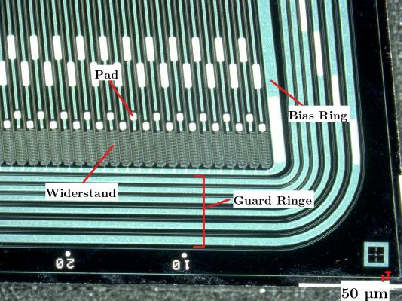
\includegraphics[width=6.5cm]{Assets/micro}
		\label{fig:micro}
		\caption{Macroscopic picture of the silicone strip sensor \cite{V15}.}
	\end{subfigure}
	\hfill
	\begin{subfigure}{0.45\textwidth}
		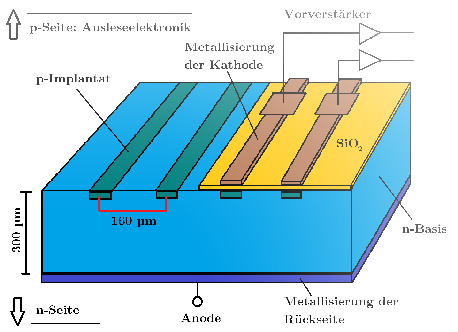
\includegraphics[width=6.5cm]{Assets/schematic}
		\caption{Schematic diagram of the silicone strip sensor\cite{V15}.}
		\label{fig:schematic}
	\end{subfigure}
\end{figure}


In the case of a not fully depleted sensor some of the electrons and holes generated by the ionizing particles are recombined outside of the depletion zone. The charge collection efficiency (CCE) describing this process when applying a laser is given by 

\begin{equation}
	\mathrm{CCE}(U)=\frac{1-\exp\left(\frac{-d_{\mathrm{c}}(U)}{a}\right)}{1-\exp\left(\frac{-D}{a}\right)},
\end{equation}
where $a$ is the penetration depth of the laser.

\subsection{Laser}
The Laser employed in this experiment is fed into the detector unit using a optic fiber cable and it has a wavelength of \qty{980}{\nano\meter}, a diameter of \qty{20}{\micro\meter}, a pulse length of \qty{5}{\nano\second} and a peak power of \qty{0.2}{\milli\watt}. The position and the focusing of the laser can be adjusted using two micrometer screws.
\subsection{Control unit}
The control unit houses the laser and is used to regulate the voltage applied to the silicone sensor. It can also measure the leakage current of the sensor. The data acquired by the control unit is transferred to the computer and can be collected there using the Alibava system.

\section{Experimental procedures}
\label{sec:exec}
Before starting the experiment it is advised to familiarize yourself with the experimental setup and the software. In the initial measurement, the current passing through the sensor is recorded at intervals of \qty{10}{\volt} for the applied voltages. This is performed until a voltage \qty{20}{\volt} above the expected depletion voltage is reached.\\

The first measurement using the software is performed in a \textit{pedestal run} of 1\,000 events, in order to determine the pedestal and noise.\\

Before using the laser or the radioactive source a set of calibration measurement is started. The fist calibration is used to determine the optimal delay. It is started using the \textit{Delay measurement} button in the Alibava software. After this run 5 different channels are used in a \textit{Calibration run}, with the applied voltage above the depletion voltage. Another run is started afterwards with the applied voltage turned down to \qty{0}{\volt}.\\

After the calibration measurement the laser is lead into the detector unit using the optic fiber cable. It is then focused and moved along the sensor until a maximally high peak is achieved in the Alibava software. Initially the optimal delay between the laser signal and the chip readout is determined using the \textit{laser sync.} function. Then the structure of the sensor is probed by recording 1\,000 events at 35 \qty{10}{\micro\meter} intervals. During the next measurements the CCE is determined by recording 1\,000 events from 0 to \qty{200}{\volt} in \qty{10}{\volt} steps.\\

A similar approach is used when measuring the radioactive source, with the difference of recording 10\,000 events per scan. \\

Finally a last scan using the radioactive source is performed and 1\,000\,000 events are recorded.
\section{Analysis}
\label{sec:Analysis}

\subsection{Depletion voltage}

\begin{figure}[H]
  \centering
  \includegraphics[height=5cm]{build/leakage.pdf}
  \caption{Measured leakage current plottet against the applied bias voltage.}
  \label{fig:leakage}
\end{figure}

\subsection{Pedestal run}

\begin{figure}[H]
  \centering
    \begin{subfigure}{0.5\textwidth}
      \includegraphics[width=\textwidth]{build/pedestal.pdf}
    \end{subfigure}
    \begin{subfigure}{0.5\textwidth}
      \includegraphics[width=\textwidth]{build/noise.pdf}
    \end{subfigure}
    \begin{subfigure}{0.5\textwidth}
      \includegraphics[width=\textwidth]{build/common_mode.pdf}
    \end{subfigure}
  \caption{TODO.}
  \label{fig:pedestal_run}
\end{figure}

\subsection{Calibration measurements}

\begin{figure}[H]
  \centering
  \includegraphics[height=5cm]{build/delay.pdf}
  \caption{TODO.}
  \label{fig:delay}
\end{figure}

\begin{figure}[H]
  \centering
  \includegraphics[height=5cm]{build/calib.pdf}
  \caption{TODO.}
  \label{fig:calib}
\end{figure}

\begin{figure}[H]
  \centering
  \includegraphics[height=5cm]{build/calib_0V.pdf}
  \caption{TODO.}
  \label{fig:calib_0V}
\end{figure}

\begin{figure}[H]
  \centering
  \includegraphics[height=5cm]{build/calib_fit.pdf}
  \caption{TODO.}
  \label{fig:calib_fit}
\end{figure}

\subsection{Measuring the strip sensor by using the laser}

\begin{figure}[H]
  \centering
  \includegraphics[height=5cm]{build/laser_delay.pdf}
  \caption{TODO.}
  \label{fig:laser_delay}
\end{figure}
\section{Discussion}
\label{sec:Discussion}

Some remarks on the analysis should be made to put the final result into more context.
While the distributions of the chosen variables show good separation, there is still room for optimization. The number of variables was arbitrarily chosen as 16,
but can easily be varied when changing the requirements on the Kolmogorov Smirnov test statistics or correlations. Testing the BDT performance with different number of
parameters could help to improve its predictive power. The five individual BDTs performed very similar, indicating that there is not too much overtraining.
However, the BDTs have all been initialized with default parameters. Tuning these parameters in a grid search could definitively help improve the BDT performance and thus
the final result.
The fits on the signal peaks have been modeled by two Gaussian functions, however they cannot describe the asymmetric shape of these peaks perfectly.
A more complicated model like a double-sided crystal ball function can improve the fit and thus directly the yield of the signal.
The significance was only estimated using \eqref{eq:sig} and seems rather high being greater than $5 \, \sigma$. Including uncertainties should help to mitigate this fact.
\section{Appendix}
\label{sec:appendix}

\begin{figure}[H]
	\centering
	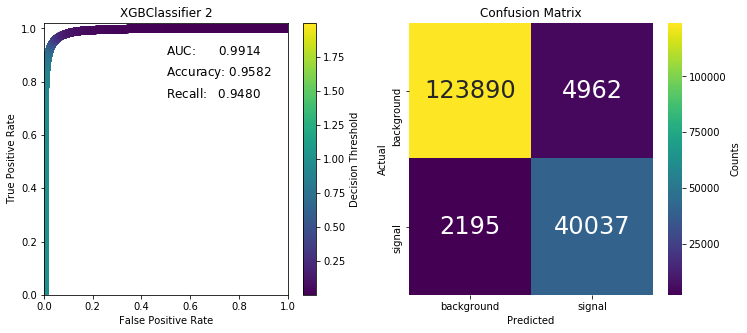
\includegraphics[width=0.8\linewidth]{plots/BDT_2.png}
	\caption{Results and scores of the second BDT.}
	\label{fig:BDT_2}
\end{figure}

\begin{figure}[H]
	\centering
	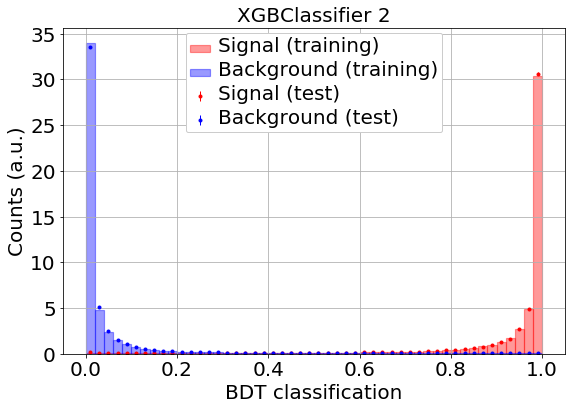
\includegraphics[width=0.5\linewidth]{plots/BDT2_pred.png}
	\caption{Response of the second BDT to training and testing data.}
	\label{fig:BDT_2_pred}
\end{figure}

\begin{figure}[H]
	\centering
	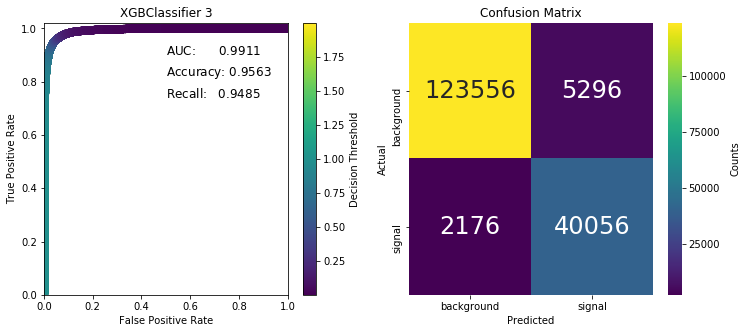
\includegraphics[width=0.8\linewidth]{plots/BDT_3.png}
	\caption{Results and scores of the third BDT.}
	\label{fig:BDT_3}
\end{figure}

\begin{figure}[H]
	\centering
	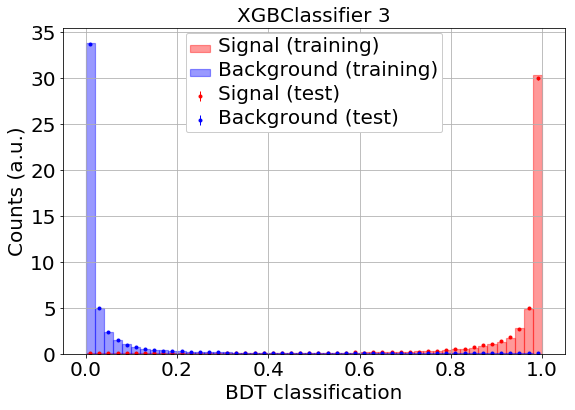
\includegraphics[width=0.5\linewidth]{plots/BDT3_pred.png}
	\caption{Response of the third BDT to training and testing data.}
	\label{fig:BDT_3_pred}
\end{figure}

\begin{figure}[H]
	\centering
	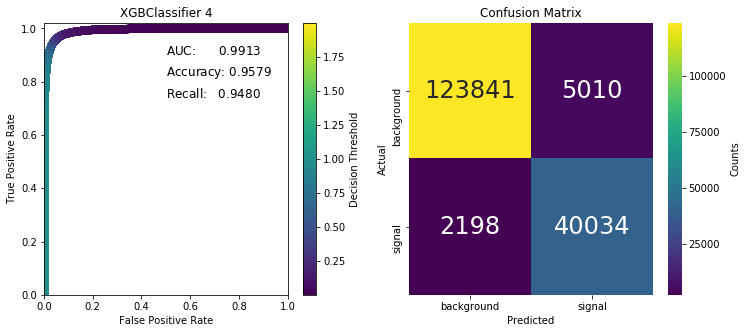
\includegraphics[width=0.8\linewidth]{plots/BDT_4.png}
	\caption{Results and scores of the fourth BDT.}
	\label{fig:BDT_4}
\end{figure}

\begin{figure}[H]
	\centering
	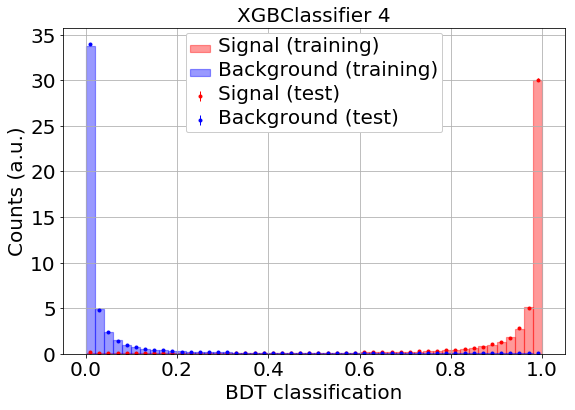
\includegraphics[width=0.5\linewidth]{plots/BDT4_pred.png}
	\caption{Response of the fourth BDT to training and testing data.}
	\label{fig:BDT_4_pred}
\end{figure}

\begin{figure}[H]
	\centering
	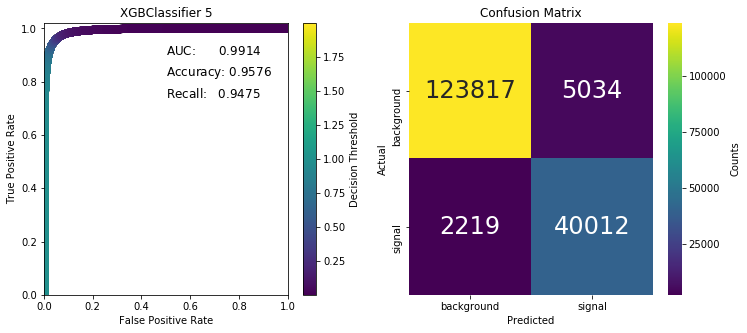
\includegraphics[width=0.8\linewidth]{plots/BDT_5.png}
	\caption{Results and scores of the fifth BDT.}
	\label{fig:BDT_5}
\end{figure}

\begin{figure}[H]
	\centering
	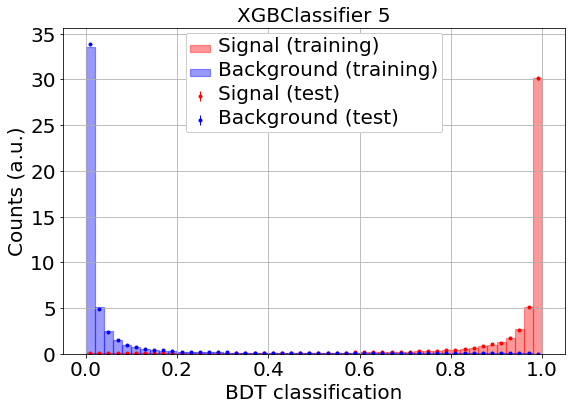
\includegraphics[width=0.5\linewidth]{plots/BDT5_pred.png}
	\caption{Response of the fifth BDT to training and testing data.}
	\label{fig:BDT_5_pred}
\end{figure}

\printbibliography{}

\end{document}
